\subsubsection{Entorno de trabajo}
El entorno de trabajo es el medio por el cuál los usuarios interactúan con la herramienta para poder gestionar la información del usuario Practicante, las rutinas, los ejercicios de calentamiento y los movimientos de técnica.
En el presente capítulo se describe el comportamiento y los elementos que conforman el entorno de trabajo de la herramienta, como son: la disposición de los elementos principales y comunes de las pantallas, los componentes, etc.\\

 \textbf{\textcolor[rgb]{0, 0, 0.545098}{Diseño}} \\

 El diseño de las pantallas de la herramienta sigue un enfoque minimalista. Las pantallas tienen un diseño homogéneo y cuentan con componentes comunes.
 En la figura \ref{fig:Entornodetrabajo} se muestran los elementos principales que conforman las pantallas de la herramienta, dichos elementos se describen a continuación:

 \begin{figure}[H]
	\centering
		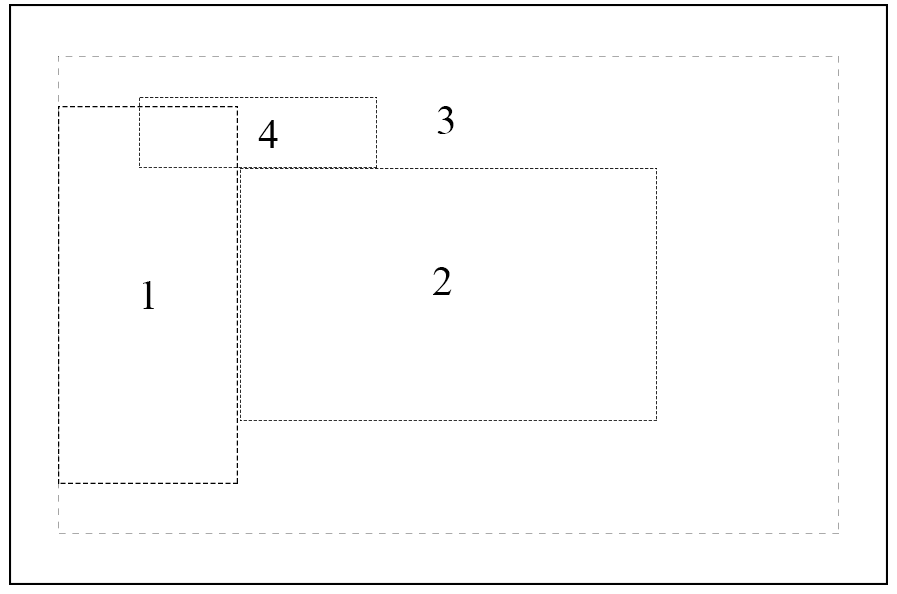
\includegraphics[scale=2]{./Figuras/Entorno_de_trabajo}
	\caption{Entorno de trabajo de la herramienta}
	\label{fig:Entornodetrabajo}
 \end{figure}
 
\begin{enumerate} 
	\item \textbf{Menú Desplegable:} es el área destinada al menú desplegable que contendrá las opciones que proporcione la herramienta, de acuerdo al elemento seleccionado.
	El menú desplegable no se encontrará visible hasta que se seleccione algún elemento y este espacio será utilizado por el área de trabajo (ver siguiente punto).
	\begin{itemize}
		\item Ancho: 300 px
		\item Alto: 466 px
	\end{itemize} 	
	
	\item \textbf{Área de Mensajes:} es el área donde aparecerán los diferentes mensajes de la herramienta (ver sección \nameref{dm:MN}).
	El mensaje no se encontrará visible hasta que la funcionalidad de la herramienta lo requiera y este espacio será utilizado por el área de trabajo (ver siguiente punto).
	\begin{itemize}
		\item Ancho: 600 px
		\item Alto: 300 px
	\end{itemize} 
	
	\item \textbf{Área de trabajo:} en esta sección los usuarios visualizarán los elementos que en la herramienta se proporcionan. Aquí se desplegarán formularios para captura, tablas y demás elementos contenidos en la herramienta.
	Todas las pantallas en esta sección deberán contar con un título alineado al centro del área de trabajo.
	\begin{itemize}
		\item Ancho: 1270 px
		\item Alto: 620 px
	\end{itemize} 
	
	\item \textbf{Información de sesión:} esta sección será visible sólo cuando un Practicante ingrese a la herramienta.
	Mostrará el nombre del Practicante y tendrá la opción para el cierre de sesión. 
	\begin{itemize}
		\item Ancho: 427 px
		\item Alto: 100 px
	\end{itemize} 
\end{enumerate}


\subparagraph{Formato de mensajes} 
Los mensajes utilizados en la herramienta se dividen en cuatro: mensajes de notificación, mensajes de confirmación, mensajes de correo electrónico y mensajes de error. \\

\textbf{\textcolor[rgb]{0, 0, 0.545098}{Mensajes de notificación}} \\

Los mensajes de notificación se muestran en pantallas emergentes, las cuales cuentan con el botón \textit{Aceptar}, que permite confirmar la lectura del mensaje, así como se muestra en la figura \ref{dm:MN}. \\

\begin{figure}[H]
	\centering
		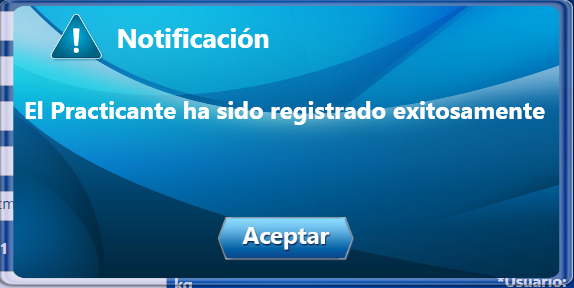
\includegraphics[scale=0.5]{./Figuras/Diseno_mensajes/Mensaje_notificacion}
	\caption{Mensaje de notificación}
	\label{dm:MN}
\end{figure}

\textbf{\textcolor[rgb]{0, 0, 0.545098}{Mensajes de confirmación}} \\

Los mensajes de confirmación se muestran en pantallas emergentes, las cuales cuentan con dos botones: \textit{Aceptar} y \textit{Cancelar}, que permiten confirmar o rechazar la acción que se muestra en el mensaje, así como se muestra en la figura \ref{dm:MC}. \\

\begin{figure}[H]
	\centering
		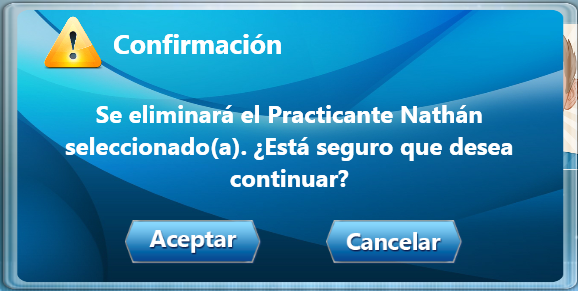
\includegraphics[scale=0.5]{./Figuras/Diseno_mensajes/Mensaje_confirmacion}
	\caption{Mensaje de confirmación}
	\label{dm:MC}
\end{figure}

\textbf{\textcolor[rgb]{0, 0, 0.545098}{Mensajes de correo electrónico}} \\

Los mensajes de correo electrónico son mandados a la dirección proporcionada por el Practicante en su registro, en ellos se escribe la información de su inicio de sesión ya sea para su nuevo registro o para el envío de una contraseña olvidada, así como se muestra en la figura \ref{dm:Correo}.  \\

\begin{figure}[H]
	\centering
		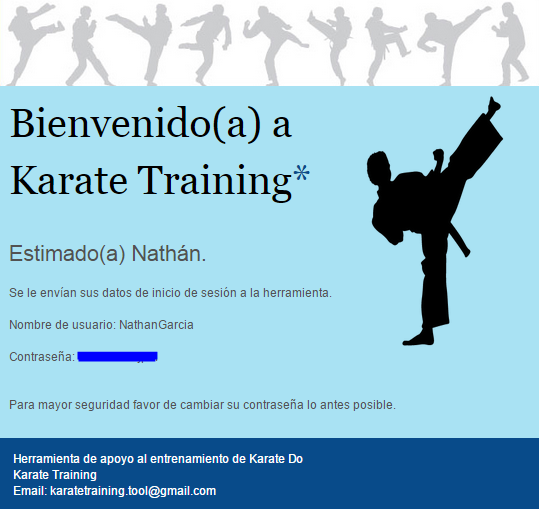
\includegraphics[scale=0.8]{./Figuras/Diseno_mensajes/Mensaje_correo}
	\caption{Mensaje de correo electrónico}
	\label{dm:Correo}
\end{figure}

\textbf{\textcolor[rgb]{0, 0, 0.545098}{Mensajes de error}} \\

Existen dos tipos de mensajes de error en la herramienta, los que se muestran en pantallas emergentes y los que muestran un identificador dentro de la misma pantalla en que se produce.\\

Los mensajes en pantallas emergentes cuentan con el botón \textit{Aceptar}, que permite confirmar la lectura del mensaje, así como se muestran en la figura \ref{dm:ME01}.\\

\begin{figure}[H]
	\centering
		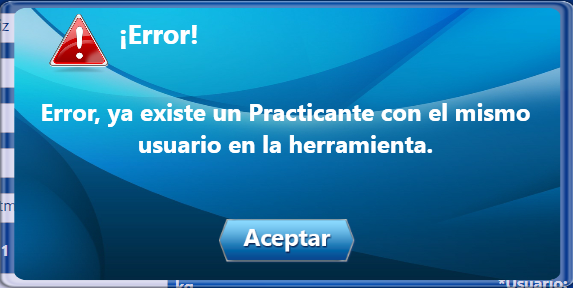
\includegraphics[scale=0.5]{./Figuras/Diseno_mensajes/Mensaje_error01}
	\caption{Mensaje de error 01}
	\label{dm:ME01}
\end{figure}

Los mensajes dentro de la misma pantalla se muestran en los campos de registro de elementos, indicando que existe un problema en dicho campo (como puede ser un formato incorrecto o un campo obligatorio que se ha dejado en blanco), la figura \ref{dm:ME02} muestra el diseño del mensaje.

\begin{figure}[H]
	\centering
		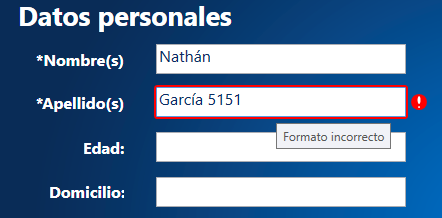
\includegraphics[scale=0.65]{./Figuras/Diseno_mensajes/Mensaje_error02}
	\caption{Mensaje de error 02}
	\label{dm:ME02}
\end{figure}